\section{Motivation and Background}
\label{background}

Figure~\ref{fig:ctas} shows the percentage of benchmarks we use in our 
evaluation that expose enough parallelism to feed larger GPUs than we have 
today. We provide additional details on the application set in 
Section~\ref{sec:methodology} and Table~\ref{tab:numctas}. More than 80\% of 
them have more CTAs (Thread Blocks) than even an 8$\times$ larger single GPU 
has Streaming Multiprocessors (SM). According to the latest Nvidia's GPU 
devices~\cite{pascal-tesla-wp}, we consider a single GPU to have 64 SMs. Such workloads would 
be able to exploit larger GPUs, with more SMs, reducing their execution time. 
Increasing a single GPU performance thus stands as a reasonable way to scale 
up the existing, as well as future applications.

Single GPU performance has been scaling very well amassing a significant
growth in per-GPU transistor count and DRAM BW. For example a 2010 Nvidia's
529mm\textsuperscript{2} Fermi GPUs integrated 1.95B transistors with 180 GB/s
DRAM bandwidth, while 2016 Nvidia 610 mm\textsuperscript{2} Pascal GPUs reached
a 12B transistor count with 720 GB/s memory bandwidth. Unfortunately transistor density
growth slows down and expected to come to a halt at 7nm. Moreover, as GPU die sizes
have been also increasing over the past generations, this growth is expected to
slow down due to limitations in lithography and manufacturing costs. 
Without larger or denser dies, GPU manufacturers are likely to turn to 
alternative technologies such as the tried and trued solution from CPU world,
the \textit{multi-socket GPUs}, to keep scaling effective GPU performance via 
growing overall transistor counts and DRAM bandwidths. 

%One moving to 3D die-stacking as a solution for continued transistor growth. 
%Unfortunately 3D die-stacking still has a significant number of engineering 
%challenges related to power delivery, energy density, and 
%cooling~\cite{verbree2010cost} when employed in maximal die-sized chips such as 
%GPUs and moving beyond a 2 high stack to 4 or 8 stacks will be even more 
%difficult. Because of these challenges, 
%GPU manufacturers are likely to 
%consider a tried and trued solution in the CPU world to gain additional 
%transistor count, \textit{multi-socket GPUs}.

\begin{figure}[t] 
    \centering
    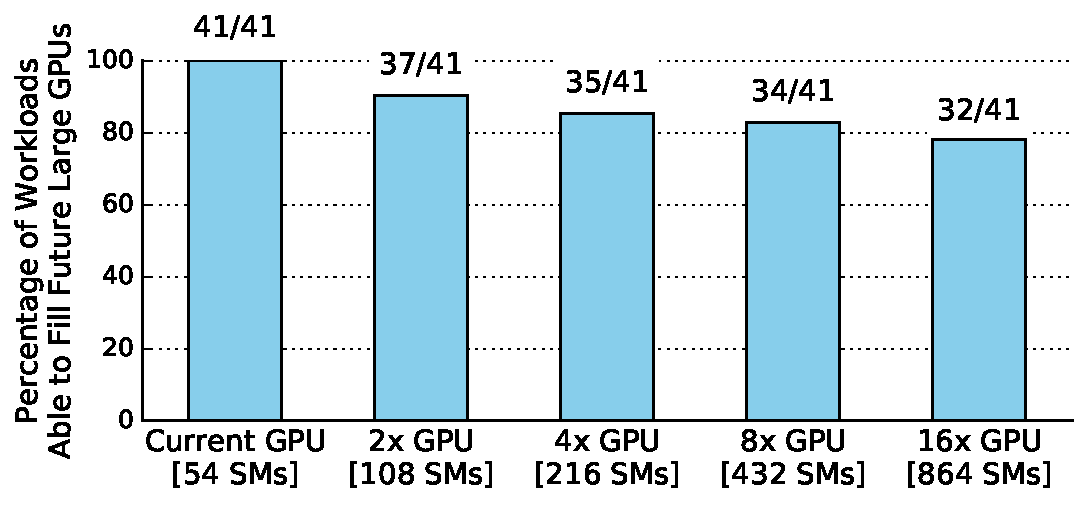
\includegraphics[width=1.0\columnwidth]{figures/plot_ctas_per_sm.pdf}
    \caption{Percentage of benchmarks that have more CTAs on average than available SMs.}
    \label{fig:ctas}
\end{figure}



The evolution of GPU computing has moved from it being a PCIe attached 
peripherals to computing platforms designed around the GPU as the primary 
computing engine. Such systems employ custom PCB designs that accommodate 
multiple high pin count socketed GPUs~\cite{dgx} with inter-GPU interconnects 
resembling QPI or Hypertransport~\cite{INTELQPI,AMDHT} much more than legacy 
PCIe interfaces.  Despite the improvement in hardware capabilities, to-date 
these multi-GPU solutions have been exposed as a collection of single GPU 
solutions with improved GPU--GPU interconnects. While multi-GPU systems can 
provide high aggregate throughput, the programming models for multi-GPU 
systems has diverged from the single GPU programming model and requires 
layering additional software runtimes like MPI or openshmem on top of the 
native GPU programming interfaces such as CUDA or openCL. By requiring 
re-writing of the GPU application to enable multi-GPU performance, many 
applications are never ported to use multiple GPUs.

In this work, we examine the performance achievable by architecting a 
multi-socket NUMA-aware single GPU.  Building upon existing work in the 
NUMA-CPU and GPU community, we first describe the basic multi-socket GPU runtime 
that allows a multi-socket GPU system to be exposed to GPU developers as a 
single GPU and exploits some well known scheduling and memory locality 
optimizations for NUMA systems. We then look at the performance implications 
that this multi-socket NUMA design has on applications that have been optimized 
for a traditional single GPU.  We identify that current GPU interconnect 
utilization and cache policies are sub-optimal for a multi-socket NUMA GPU and 
show how these problems can largely be overcome with architectural innovation.  
Finally, we examine the scaling efficiency of a multi-socket NUMA-aware GPU to 
understand if NUMA-aware GPUs will see significantly improve performance  
without any code-rewriting required by the application programmer.


----------Evgeny ---- 
the following paragraphs moved from next section, need to be merged here or in
Intro ----------

To improve the performance of our
basic TMS-GPU implementation we propose two classes of improvements that 
leverage application phasing to reduced the effective NUMA penalty.  First, in 
Section~\ref{interconnect} we examine the ability of a switch connected GPU to 
dynamically change its interconnect signaling from a balanced up and down 
stream bandwidth design, to allowing flexible re-partitioning of these channels.  
When bi-directional bandwidth is observed to be under-utilized, the direction 
which has excess capacity can be re-assigned to support the oversubscribed 
channels. This allows any individual GPU to improve its bandwidth utilization at 
times when it finds itself most bandwidth constrained.

Second, because we observe that inter-GPU bandwidth has a strong correlation to
overall multi-socket GPU performance we investigate the performance impact of
enabling multi-socket GPU cache coherence in Section~\ref{caching}.  We propose
extending the software based L1 coherence into the L2 caches of multi-socket
GPUs.  By extending this coherence, the L2 caches of each GPU socket move from
being memory-side, where coherence is not needed, to GPU-side, where coherence
guarantees are required in the same manner as current GPU L1 caches.  We
evaluate the effect of this coherence overhead on multi-socket GPUs and show
that because of the GPU's weak coherence guarantees multi-socket coherence on
GPUs should scale significantly better than traditional CPU coherence
protocols.

Finally, we show that after extending coherence into the GPU L2 caches, the
appropriate allocation of cache capacity between local memory bandwidth and
remote memory bandwidth can not be decided at design time.  Due to the same
application phasing that enabled dynamic interconnect re-balancing, we observe
that individual GPU sockets should be free to balance their cache capacity
between local and remote accesses to optimize performance.  When remote
interconnect bandwidth is saturated, a GPU will skew its cache capacity toward
the remote accesses,  however if that bandwidth is not saturated then
optimizing cache hit rates to eliminate the largest number of memory requests
is desirable.

Before diving into detailed proposals and results for our proposed
optimizations we first describe the TMS-GPU runtime that consolidates
prior work from both the NUMA-GPU world and GPU then describe our multi-socket
GPU methodology.

\begin{figure*}[tp] 
    \centering
    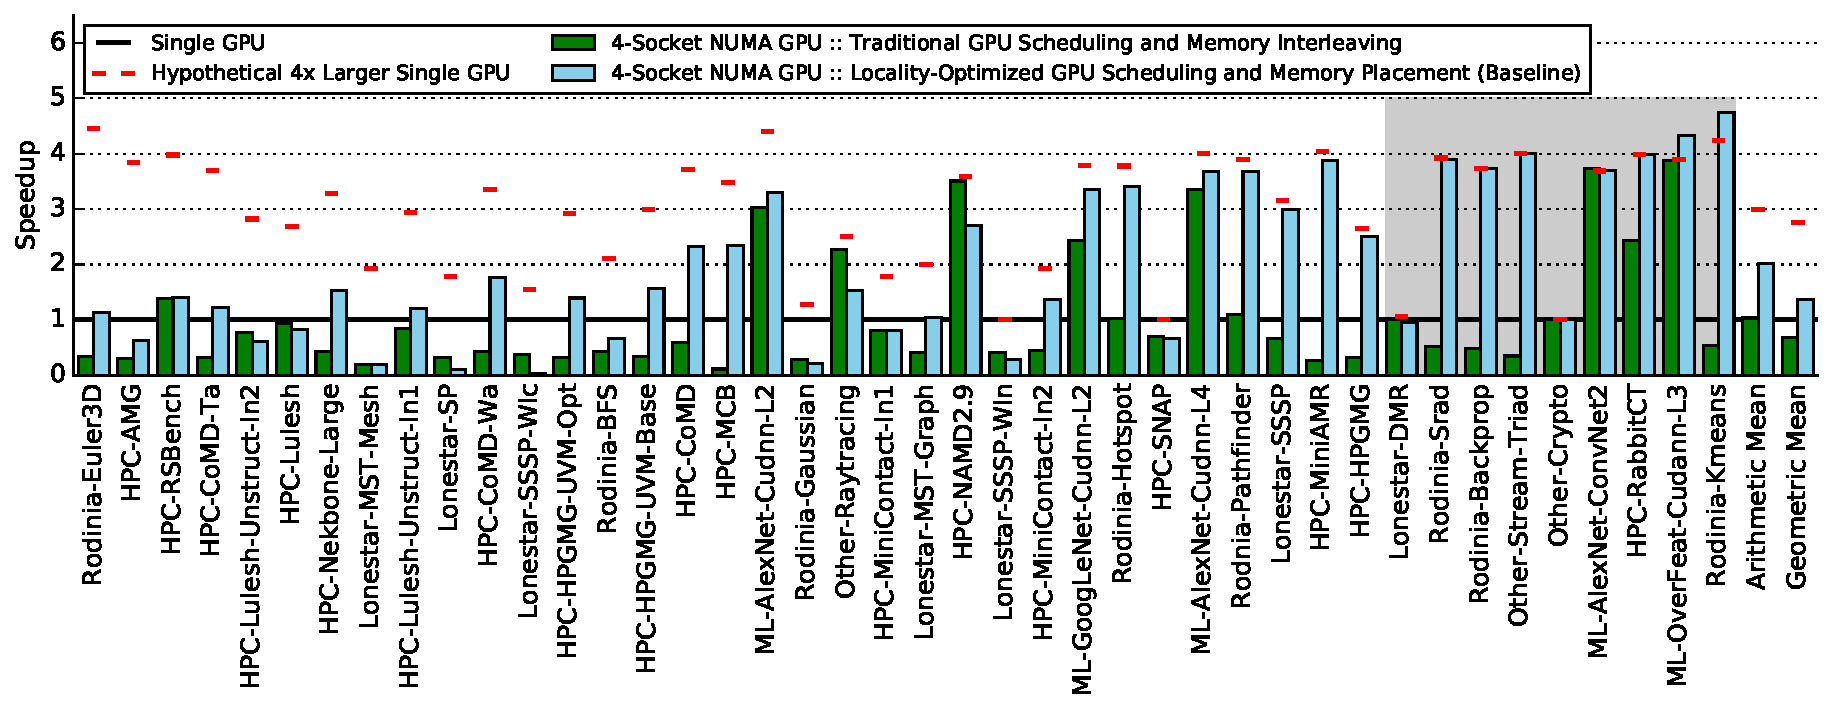
\includegraphics[width=1.0\linewidth]{figures/plot_different_baselines.pdf}
    \caption{Relative performance of a 4-socket NUMA GPU using to a single GPU 
and a hypothetical 4$\times$ larger (all resources scaled) single GPU showing 
upper bound of performance this application can achieve via GPU hardware 
scaling. For the Locality-Optimized design, applications shown in grey 
achieve already 99\% of theoretical scaling (\emph{red dash}) without 
micro-architectural modification.}
    \label{fig:motivation}
\end{figure*}
